\documentclass{beamer}

\usetheme{CambridgeUS}

\usepackage[utf8]{inputenc}
\usepackage[T1]{fontenc}

\usepackage{CJKutf8}
\usepackage{datetime}
\usepackage{amsmath}
\usepackage{amssymb}
\usepackage{mathtools}
\usepackage{subcaption}
\usepackage{minted}
\usepackage{xcolor}
\usepackage{ulem}
\usepackage{hyperref}
\usepackage{graphicx}
\usepackage{cite}
\usepackage{multirow}
\usepackage{makecell}
\usepackage{url}
\usepackage{placeins}

\graphicspath{{images/}}
\DeclareGraphicsExtensions{.pdf}

\newdate{date}{30}{08}{2024}
\date{\displaydate{date}}
\title[Fairness]{Ensuring Fairness with Transparent Auditing of
Quantitative Bias in AI Systems}
\author[Rex]{
    \begin{CJK}{UTF8}{bsmi}袁至誠\end{CJK}\newline
    Chih-cheng Rex Yuan\newline
    \href{https://rexyuan.com/}{rexyuan.com}
    }
\institute[IIS,AS]{Institute of Information Science, Academia Sinica}

\DeclarePairedDelimiter{\set}{\{}{\}}
\DeclarePairedDelimiter{\tuple}{(}{)}
\DeclarePairedDelimiter{\abs}{\lvert}{\rvert}

\let\oldleq\leq
\renewcommand{\leq}[1][]{\oldleq_{#1}}
\renewcommand{\implies}{\rightarrow}

\newcommand{\bye}[1]{}

\newcommand{\red}[1]{\textcolor{red}{#1}}
\newcommand{\sred}[1]{\textcolor{red}{\sout{#1}}}

\begin{document}

\begin{frame}
\titlepage
\end{frame}

\begin{frame}
    \frametitle{AI Bias}
    \begin{itemize}
        \item AI is widely used in decision making:
        \begin{itemize}
            \item School admission.
            \item Loan approval.
            \item Hiring.
            \item Policing.
            \item Censorship.
            \item etc..
        \end{itemize}
        \item Decision making by AI may be biased.
        \item Bias can come from several sources:
        \begin{itemize}
            \item Biased data. ML is deisgned to replicate this.
            \item Missing data. The datasets might not be representative.
            \item Biased algorithms. The objective functions might introduce bias.
            \item Sensitive attributes: Age, Gender, ..., etc..
        \end{itemize}
    \end{itemize}
\end{frame}

\begin{frame}
    \frametitle{Protected Attributes}
    What are the protected(sensitive) attributes?
    \begin{table}
        \begin{tabular}{|c|c|c|c|c|}
            \hline
            \red{Age} & \red{Gender} & Occupation & \red{Income} & Education \\
            \hline
            \red{28} & \red{M} & Engineering & \red{\$80,000} & Master \\
            \red{28} & \red{F} & Engineering & \red{\$65,000} & Master \\
            \red{45} & \red{M} & Medicine    & \red{\$100,000} & Doctorate \\
            \red{40} & \red{F} & Legal       & \red{\$150,000} & Law Degree \\
            \red{32} & \red{M} & Education   & \red{\$55,000} & Bachelor \\
            \hline
        \end{tabular}
        \caption{Example Dataset}
    \end{table}
\end{frame}

\begin{frame}
    \frametitle{Fairness Through Unawareness}
    The most straightforward solution to fairness seems to be that
    just simply dropping all the protected columns.
    \begin{itemize}
        \item This is called fairness through unawareness.
        \item Formally it's
        \[
            X_i = X_j \implies \hat{Y}_i = \hat{Y}_j
        \]
        where $i,j$ are individuals; $X$ is the set of attributes
        except protected attributes; and $\hat{Y}$ is the prediction.
        \item Also known as fairness through blindness and
        anti-classification.
    \end{itemize}
\end{frame}

\begin{frame}
    \frametitle{Fairness Through Unawareness}
    The downside of this is there could still be ``proxy'' attributes
    that correlate with protected attributes: like Occupation still
    correlates with Income.
    \begin{table}
        \begin{tabular}{|c|c|c|c|c|}
            \hline
            \sout{Age} & \sout{Gender}   & \red{Occupation}  & \red{\sout{Income}}   & Education \\
            \hline
            \sout{28} & \sout{M} & \red{Engineering} & \red{\sout{\$80,000}} & Master \\
            \sout{28} & \sout{F} & \red{Engineering} & \red{\sout{\$65,000}} & Master \\
            \sout{45} & \sout{M} & \red{Medicine}    & \red{\sout{\$100,000}} & Doctorate \\
            \sout{40} & \sout{F} & \red{Legal}       & \red{\sout{\$150,000}} & Law Degree \\
            \sout{32} & \sout{M} & \red{Education}   & \red{\sout{\$55,000}} & Bachelor \\
            \hline
        \end{tabular}
        \caption{Example Dataset}
    \end{table}
\end{frame}

\begin{frame}
    \frametitle{Demographic Parity}
    Formally, it requires that
    \[
        \abs{P[\hat{Y} = 1 | S = 1] - P[\hat{Y} = 1 | S \neq 1]} \leq \epsilon
    \]
    where $\hat{Y} = 1$ represents acceptance(positive);
    $S = 1$ represents privileged group;
    $S \neq 1$ represents unprivileged group where $S$ is some protected
    attributes.

    Let's set $\epsilon = 0.2$.
    If for some job opening, male is the privileged group and
    there are $10$ female applicants and
    $100$ male applicants, and there are $8$ accepted females
    and $90$ accepted males:
    \[
        \abs{8/10 - 90/100} = 0.1 < \epsilon \quad\text{so this is fair}
    \]
    while if there were $1$ accepted females and $50$ accepted males:
    \[
        \abs{1/10 - 50/100} = 0.4 > \epsilon \quad\text{so this is unfair}
    \]
\end{frame}

\begin{frame}
    \frametitle{Disadvantages of Demographic Parity}
    \begin{itemize}
        \item A fully accurate classifier
        may be considered unfair.
        \item The notion permits that we accept the qualified applicants in
        one demographic, but random individuals in another, so long as the
        percentages of acceptance match.
        \item For example, the case with 90 qualified males and only 1
        qualified females.
    \end{itemize}
\end{frame}

\begin{frame}
    \frametitle{Equalized Odds}
    \begin{itemize}
        \item Equalized odds is designed to address the downsides of the previous two
        by taking into accounts the ``ground truths'' and consider
        the difference between false-positive rates and true-positive rates of
        the groups.
        \item Formally, it requires that
        \begin{align*}
            \abs{P[\hat{Y} = 1 | S = 1, Y = 0] - P[\hat{Y} = 1 | S \neq 1, Y = 0]} & \leq \epsilon \\
            \abs{P[\hat{Y} = 1 | S = 1, Y = 1] - P[\hat{Y} = 1 | S \neq 1, Y = 1]} & \leq \epsilon
        \end{align*}
        where $Y$ represents ground truths.
        \item A fully accurate classifier
        will necessarily satisfy the two equalized odds constraints.
    \end{itemize}
\end{frame}

\begin{frame}
    \frametitle{Equal Opportunity}
    \begin{itemize}
        \item It is a relaxation of equalized odds.
        \item Formally, it requires that
        \begin{align*}
            \abs{P[\hat{Y} = 1 | S = 1, Y = 1] - P[\hat{Y} = 1 | S \neq 1, Y = 1]} & \leq \epsilon
        \end{align*}
        where $Y$ represents ground truths.
    \end{itemize}
\end{frame}

\begin{frame}
    \frametitle{COMPAS}
    \textbf{recidivism} \textit{noun} \\
    \quad the tendency of a convicted criminal to reoffend.
    \begin{columns}[T]
        \begin{column}{.5\textwidth}
            \centering
            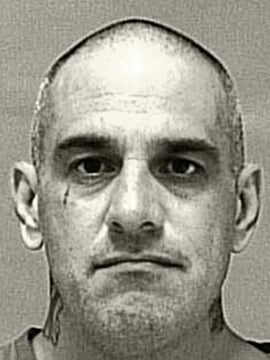
\includegraphics[width=.5\textwidth]{PRATER.jpg}
            \footnotesize
            \begin{itemize}
                \item Prior Offenses: 2 armed robberies, 1 attempted armed robbery
                \item Subsequent Offenses: 1 grand theft
                \item Risk Score: 3
            \end{itemize}
        \end{column}
        \begin{column}{.5\textwidth}
            \centering
            
\includegraphics[width=.5\textwidth]{BORDEN.jpg}
            \footnotesize
            \begin{itemize}
                \item Prior Offenses: 4 juvenile misdemeanors
                \item Subsequent Offenses: None
                \item Risk Score: 8
            \end{itemize}
        \end{column}
    \end{columns}
\end{frame}

\begin{frame}
    \frametitle{COMPAS}
    \begin{itemize}
        \item COMPAS is an algorithm
        used by U.S. courts for predicting recidivism based on a
        questionaire and background information.
        \item In 2016, ProPublica found that the algorithm is biased.
        \begin{quote}
            Black defendants were often predicted to be at a higher risk of recidivism than they actually were.
            White defendants were often predicted to be less risky than they were.
        \end{quote}
        \item The false-positive rates vary significantly across
        black people and white people, violating equalized odds.
        \item Supreme Court ruled that it can be considered by judges during
        sentencing, but there must be warnings about the tool's "limitations and cautions."
    \end{itemize}
    \footnotetext[1]{\href{https://www.propublica.org/article/how-we-analyzed-the-compas-recidivism-algorithm}{(Link) ProPublica - How We Analyzed the COMPAS Recidivism Algorithm}}
    \footnotetext[2]{\href{https://www.youtube.com/watch?v=TqnYf2h6A-k}{(Link) Vsauce2 - The Dangerous Math Used To Predict Criminals}}
\end{frame}

\begin{frame}
    \frametitle{Other Measures}
        \begin{table}[h]
            \centering
            \resizebox{0.93\textwidth}{!}{
            % \resizebox{\columnwidth}{!}{
            \begin{tabular}{|l|c|} % 'l' specifies left alignment for the first column
                \hline
                \textbf{Fairness Measure} & \textbf{Definition} \\
                \hline
        Disparate Impact & $\frac{P[\hat{Y} = 1 | S \neq 1]}{P[\hat{Y} = 1 | S = 1]} \geq 1 - \epsilon$ \\
        \hline
        Demographic Parity & $\abs{P[\hat{Y} = 1 | S = 1] - P[\hat{Y} = 1 | S \neq 1]} \leq \epsilon$ \\
        \hline
        Conditional Statistical Parity & $\abs{P[\hat{Y} = 1 | S = 1, L = l] - P[\hat{Y} = 1 | S \neq 1, L = l]} \leq \epsilon$ \\
        \hline
        Overall Accuracy Equality & $\abs{P[Y = \hat{Y} | S = 1] - P[Y = \hat{Y} | S \neq 1]} \leq \epsilon$ \\
        \hline
        Mean Difference & $\abs{E[\hat{Y}|S = 1] - E[\hat{Y}|S \neq 1]} \leq \epsilon$ \\
        \hline
        \multirow{2}{*}{Equalized Odds} & $\abs{P[\hat{Y} = 1 | S = 1, Y = 0] - P[\hat{Y} = 1 | S \neq 1, Y = 0]} \leq \epsilon$ \\
        \cline{2-2}
                                        & $\abs{P[\hat{Y} = 1 | S = 1, Y = 1] - P[\hat{Y} = 1 | S \neq 1, Y = 1]} \leq \epsilon$ \\
        \hline
        Equal Opportunity & $\abs{P[\hat{Y} = 1 | S = 1, Y = 1] - P[\hat{Y} = 1 | S \neq 1, Y = 1]} \leq \epsilon$ \\
        \hline
        Predictive Equality & $\abs{P[\hat{Y} = 1 | S = 1, Y = 0] - P[\hat{Y} = 1 | S \neq 1, Y = 0]} \leq \epsilon$ \\
        \hline
        \multirow{2}{*}{Conditional Use Accuracy Equality} & $\abs{P[Y = 1 | S = 1, \hat{Y} = 1] - P[Y = 1 | S \neq 1, \hat{Y} = 1]} \leq \epsilon$ \\
        \cline{2-2}
                                         & $\abs{P[Y = 0 | S = 1, \hat{Y} = 0] - P[Y = 0 | S \neq 1, \hat{Y} = 0]} \leq \epsilon$ \\
        \hline
        Predictive Parity & $\abs{P[Y = 1 | S = 1, \hat{Y} = 1] - P[Y = 1 | S \neq 1, \hat{Y} = 1]} \leq \epsilon$ \\
        \hline
        Equal Calibration & $\abs{P[Y = 1 | S = 1, \hat{V} = v] - P[Y = 1 | S \neq 1, \hat{V} = v]} \leq \epsilon$ \\
        \hline
        Positive Balance & $\abs{E[\hat{V} | Y = 1, S = 1] - E[\hat{V} | Y = 1, S \neq 1]} \leq \epsilon$ \\
        \hline
        Negative Balance & $\abs{E[\hat{V} | Y = 0, S = 1] - E[\hat{V} | Y = 0, S \neq 1]} \leq \epsilon$ \\
        \hline
            \end{tabular}
            }
            \caption{Fairness measures.}
            \label{tab:measures}
        \end{table}
\end{frame}

\begin{frame}
    \frametitle{Framework}
    We made a tool to calculate these measures.

    Our framework consists of 3 parties: data provider, model maker, and auditor.
    \begin{itemize}
        \item Data provider has access to the real world data.
        For example, a census bureau.
        \item Model maker designs AI models that is to be used on data.
        They can use our tool on their in-house data to test their models.
        \item Auditor is some 3rd-party that takes real data and a model or
        model result.
        They can use our tool to determine the fairness of the model.
    \end{itemize}
\end{frame}

\newcommand{\db}{\mathcal{D}}
\newcommand{\model}{\mathcal{M}}
\newcommand{\priv}{R}
\newcommand{\pos}{\hat{P}}
\newcommand{\posm}{\hat{P}_\mathcal{M}}
\newcommand{\tru}{T}
\newcommand{\leg}{L}
\newcommand{\sco}{\hat{S}}
\newcommand{\scom}{\hat{S}_\mathcal{M}}
\newcommand{\calib}{C}

\begin{frame}
    \frametitle{Predicate}
    We first introduce the idea of a predicate.
    \begin{itemize}
        \item A \emph{predicate} is a decider that determines
        if some condition holds for some given input.
        \item Formally, it is a function that takes
        some type $\alpha$ and returns True or False.
        \item For example, an ``$\text{adult}(x)$'' predicate might
        take a person $x$'s data and returns if they are over 18
        year old.
    \end{itemize}
\end{frame}

\begin{frame}
    \frametitle{Abstraction}
    Our framework tool abstracts the fairness measures:
    \begin{itemize}
        \item A \emph{row} is a lookup table or dictionary.
        $r_n(\text{``sex''}) = \text{``Female''}$ means $r_n$'s sex is female.
        \item A \emph{privileged predicate} $\priv$ takes a row and determines if
        it belongs to the privileged group.
        For example, $\priv(r_i) := r_i(\text{``race''}) == \text{``Caucasian''}$
        means the privileged group is those with race being Caucasian.
        \item A \emph{positive predicate} $\pos$ takes a row and determines if its
        prediction is positive. For example,
        $\pos(r_i) := \mathtt{int}(r_i(\text{``score''})) > 7$ means a
        row's prediction is positive if its score is greater than 7.
        \item A \emph{ground truth predicate} $\tru$ takes a row and gives the ground
        truth of the result. For example,
        $\tru(r_i) := r_i(\text{``recid''}) == \text{True}$ indicates a
        row's actual recidivism.
    \end{itemize}
\end{frame}

\begin{frame}
    \frametitle{Definition}
    We can use these abstractions to define fairness measures.
    For equal opportunity, recall its formal definition:
    \begin{align*}
        \abs{P[\hat{Y} = 1 | S = 1, Y = 1] - P[\hat{Y} = 1 | S \neq 1, Y = 1]}
        \leq \epsilon
    \end{align*}
    To model $Y$, $\hat{Y}$, and $S$, we define the corresponding
    $\tru$, $\pos$, and $\priv$.
    \begin{itemize}
        \item $Y = 1$ if and only if $\tru$ is true
        \item $\hat{Y} = 1$ if and only if $\pos$ is true
        \item $S = 1$ if and only if $\priv$ is true
        \item and vice versa
    \end{itemize}
    This way, we can calculate equal opportunity as a function:
    \begin{align*}
        \text{equal\_opportunity} (\epsilon, \priv, \pos, \tru)
    \end{align*}
\end{frame}

\begin{frame}[fragile]
    \frametitle{Definition}
    \begin{align*}
        \text{equal\_opportunity} (\epsilon, \priv, \pos, \tru)
    \end{align*}

    This is implemented in our tool as a Python function:

    \begin{center}
    \begin{minipage}{0.8\textwidth}
    \begin{minted}[fontsize=\small, frame=single, linenos]{python}
def equal_opportunity(
    ratio,
    privileged_predicate,
    positive_predicate,
    truth_predicate):
    ...
    \end{minted}
    \end{minipage}
    \end{center}
\end{frame}

\begin{frame}
    \frametitle{Application}
    For demonstration, we analyzed the COMPAS dataset.
    Let's set the predicates:
    \begin{align*}
        \priv(r_i) & := r_i(\text{``race''}) \neq \text{``African-American''}\\
        \pos(r_i)  & := r_i(\text{``score\_text''}) \in \set{\text{``Medium''},\text{``High''}}\\
        \tru(r_i)  & := r_i(\text{``two\_year\_recid''}) == \text{True}
    \end{align*}
    These predicates can be published for transparency.
\end{frame}

\begin{frame}[fragile]
    \frametitle{Application}
    \begin{align*}
        \priv(r_i) & := r_i(\text{``race''}) \neq \text{``African-American''}\\
        \pos(r_i)  & := r_i(\text{``score\_text''}) \in \set{\text{``Medium''},\text{``High''}}\\
        \tru(r_i)  & := r_i(\text{``two\_year\_recid''}) == \text{True}
    \end{align*}
    These predicates can then be encoded with Python functions:
    \begin{center}
    \begin{minipage}{0.8\textwidth}
    \begin{minted}[fontsize=\small, frame=single, linenos]{python}
equal_opportunity(
    0.2,
    lambda row: row['race'] != 'African-American',
    lambda row: row['score_text']
      in {'Medium', 'High'},
    lambda row: row['is_recid'] == '1')
    \end{minted}
    \end{minipage}
    \end{center}
\end{frame}

\begin{frame}
    \frametitle{Application}
    \centering
    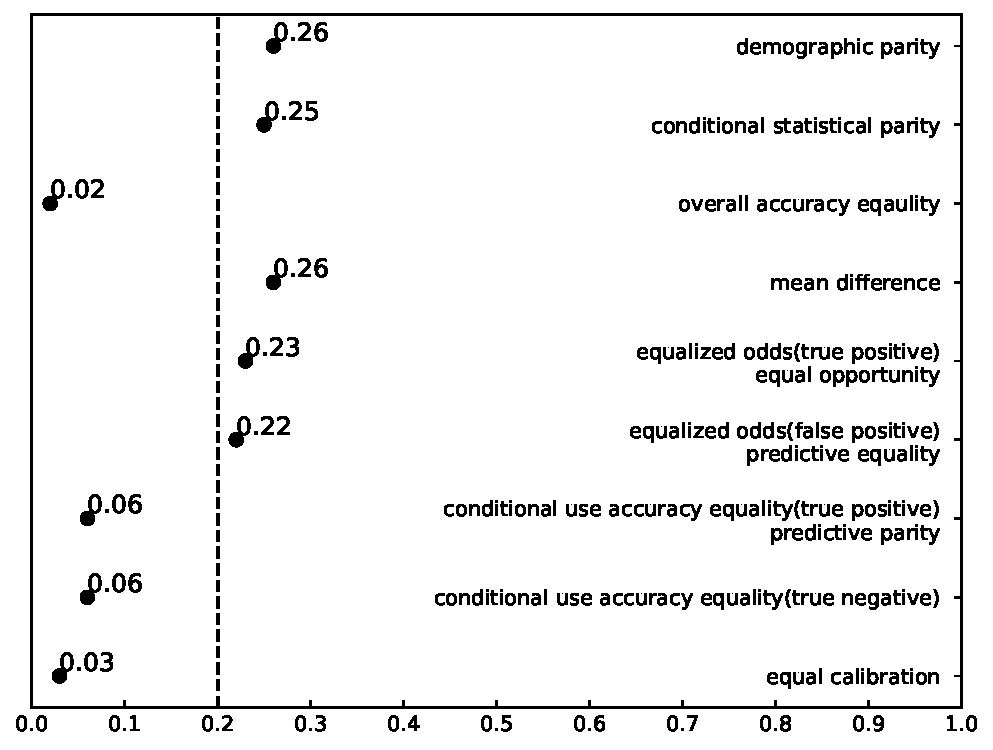
\includegraphics[width=0.73\textwidth]{African-American}
    \captionof{figure}{Unprivileged Group: African-American}
\end{frame}

\begin{frame}
    \frametitle{Application}
    \centering
    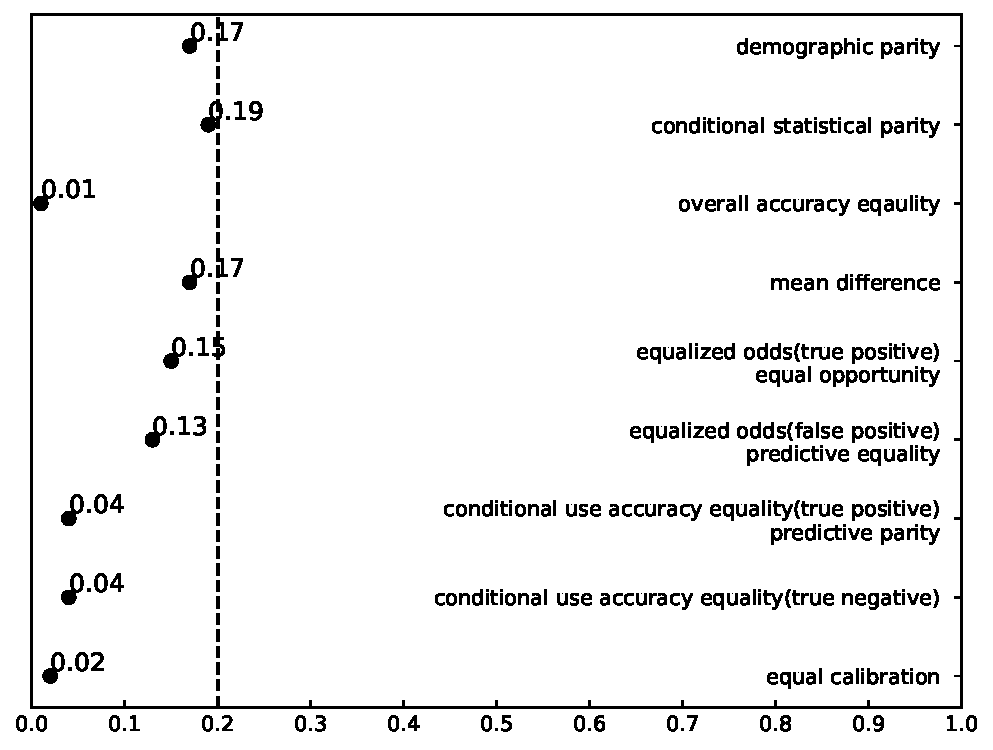
\includegraphics[width=0.73\textwidth]{Caucasian}
    \captionof{figure}{Unprivileged Group: Caucasian}
\end{frame}

\begin{frame}
    \frametitle{Application}
    \centering
    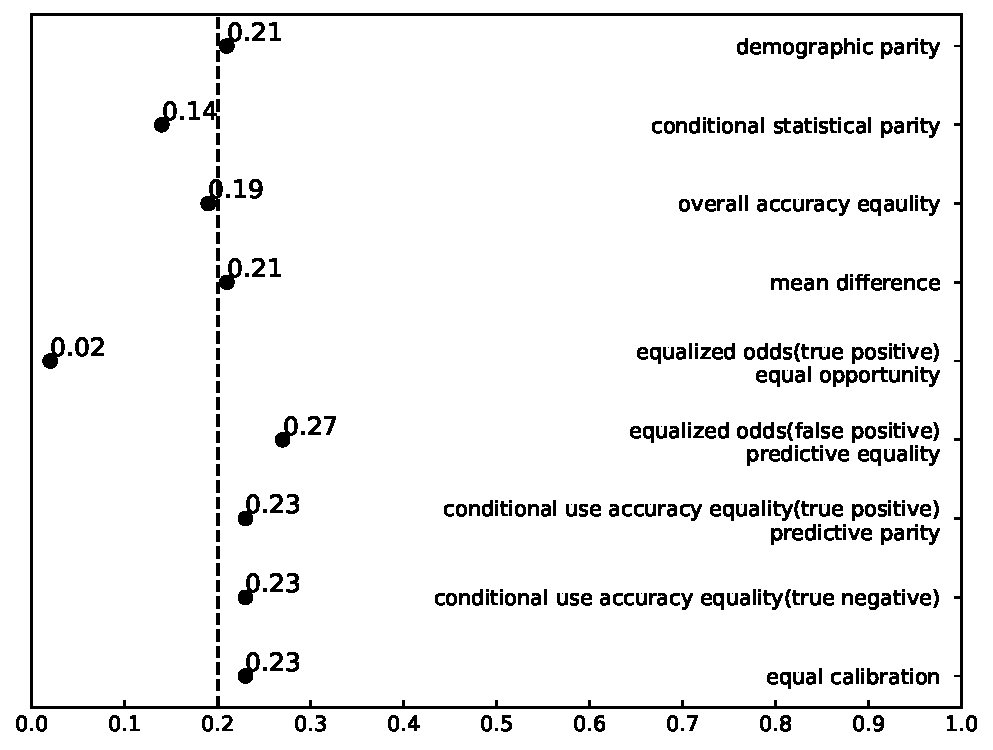
\includegraphics[width=0.73\textwidth]{Asian}
    \captionof{figure}{Unprivileged Group: Asian (32 rows)}
\end{frame}

\begin{frame}
    \frametitle{Conclusion}
    \begin{itemize}
        \item Decision making by AI may be biased.
        \item With our framework tool, auditors can comprehensively
        review the fairness of an AI system.
    \end{itemize}

    This slides is available at \url{https://github.com/RexYuan/Shu}.
\end{frame}

\end{document}
